\chapter{Background}
% A more extensive coverage of what's required to understand your work.

% In general you should assume the reader has a good undergraduate
% degree in computer science, but is not necessarily an expert in the
% particular area you've been working on. Hence this chapter may need to
% summarize some ``text book'' material.
%
% This is not something you'd normally require in an academic paper, and
% it may not be appropriate for your particular circumstances. Indeed,
% in some cases it's possible to cover all of the ``background''
% material either in the introduction or at appropriate places in the
% rest of the dissertation.
%

\section{Online Schedulers}
\begin{tcolorbox}[boxsep=0mm,left=2.5mm,right=2.5mm] \textbf{Online Schedulers:}
{\em This chapter formalises the scheduling problem as well as highlighting the
additional challenges of online scheduling vs offline scheduling. In addition,
it will list existing scheduler taxonomies, highlighting their use cases,
advantages and disadvantages.}  \end{tcolorbox}

\section{Kubernetes Overview}

\begin{figure}[h]
    \centering
    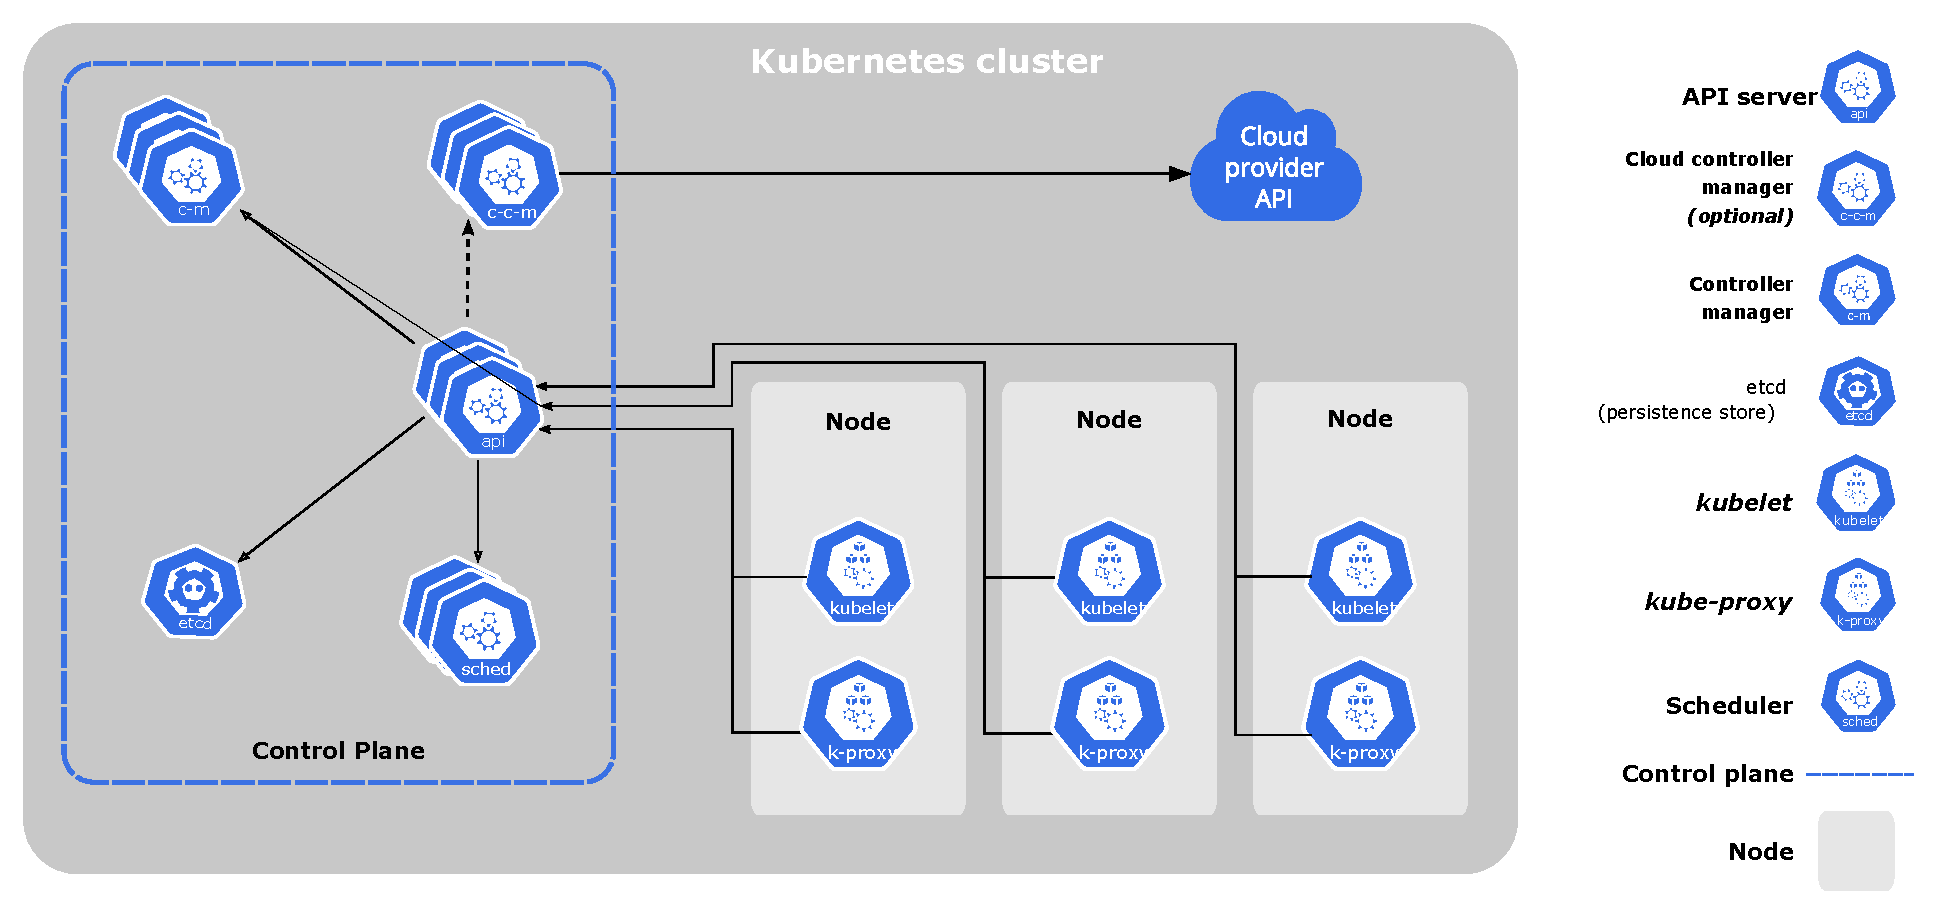
\includegraphics[width=\textwidth]{images/components-of-kubernetes.pdf}
    \caption{The components of a Kubernetes cluster}
    \label{kube-components}
\end{figure}

A Kubernetes cluster consists of a control plane and one or more worker nodes.
Components in the control plane manage the overall state of the cluster. The
\verb|kube-apiserver| exposes the Kubernetes HTTP API, which is used to publish
objects such as Deployments, DaemonSets and Jobs. The \verb|kube-server| looks
for pods not yet bound to a pod, and assigns each Pod to a suitable node. Each
node in the cluster contains a set of components which maintain the running pods
and provide the Kubernetes runtime environment. \verb|kubelet| manages Pods and
ensures they and their containers are running. The \verb|kubelet| uses a
container runtime: software responsible for running containers.

Kubernetes objects are persistent entities in the Kubernetes system. They act as
"records of intent" and describe the cluster's desired state: once created, the
Kubernetes system will constantly work to ensure that the objects exists. The
Kubernetes API is used to create, modify or delete Kubernetes objects. Almost
every Kubernetes object includes two fields: \verb|spec| and \verb|status|.
\verb|spec| is used on creation as a description of the characteristics you want
the resource to have, while \verb|status| describes the current state of the
object, supplied and updated by the Kubernetes system. These fields are crucial
for scheduling pods as they behave like resource constraints, with which the
Kubernetes schedulers can use to determine optimal pod placement.

\section{Analysis of Scheduling Approaches and QoS-Aware Trends}
Different Kubernetes schedulers take varied approaches to plod placement, from
simple heuristics to global optimisations and machine learning. This diversity
reflects the wide range of workload requirements and cluster scales seen in
practice. In the following subsections, we compare how different schedulers
leverage different data inputs for decision-making, which fundamentally
influences their scheduling strategy and resulting quality of service (QoS) for
workloads.

\subsection{Pod Spec-Only Scheduling vs Telemetry-Aware Scheduling}

\textbf{Pod Description-Based schedulers} rely solely on the information declared
in the pod specification and cluster configuration (static data). The default
Kubernetes scheduler \cite{} and similar schedulers like Yunikorn or Volcano
\cite{} fall in this category. They consider factors such as requested
CPU/memory, labels and selectors, affinity/anti-affinity rules, and priority.
This approach is more reliable for ensuring that the declared needs of a pod are
met. For example, a pod will only be placed on a node that has enough free
capacity according to a resource requests, and it will honour policies like zone
spreading or node affinity.

Benefits of this method are predictability and
simplicity: by using static reservations, the scheduler guarantees that if every
pod accurately requests its needs, no node will be over-committed at scheduling
time. This can protect critical workloads by giving them guaranteed resources
(as in Kubernetes Guaranteed QoS class). It also enables fairness policies at
high level (e.g. Yunikorn's queues and priorities ensure no team monopolises the
cluster).

However, the downside is a lack of visibility into actual runtime conditions -
the scheduler is blind to fluctuations in load or hardware state. As a result,
static-only scheduling may lead to less optimal placements: for instance, a new
pod might be placed on a node that technically has room (per requests) but is
currently experience high CPU utilisation from other processes, leading to
contention. Meanwhile, an underutilised node could be ignored because its
capacity appears full due to over-requested resources or sticky allocations. In
summary, purely \verb|spec|-based scheduling treats the cluster as a static
partitioning of resources; it ensures each workload's declared needs are met, but
it can't respond to real-time performance variations.

\textbf{Telemetry-Based schedulers}, incorporate live metrics and feedback from
the cluster's current state to make more informed decisions. These schedulers
actively monitor CPU usage, memory pressure, I/O rates, cache misses, network
latency, etc., either via the Kubernetes Metrics APU, Prometheus, or custom
telemetry pipelines. Examples include Intel's Telemetry Aware Scheduling \cite{}
(which uses fine-grained platform metrics like LLC cache hit rates and CPU
temperature) and the Trimaran plugin suite for Kubernetes \cite{} that uses
real-time utilisation stats.

By using this data, telemetry-driven scheduling can avoid placing pods on nodes
that are struggling or overloaded in real-time. For instance, a telemetry-aware
scheduler might detect that Node A's CPU is 90\% busy and Node B's is 20\% and
therefore prefer Node B for a new pod - even if, by static allocation, both
nodes had equal allocable capacity remaining. This dynamic adaptability
directly improves QoS: workloads get more stable performance because they are
less likely to be scheduled to an over-taxed machine. Moreover, telemetry-based
rules can target specific QoS concerns: Intel's TAS can steer latency-sensitive
network functions away from nodes with high cache thrashing, preventing
unpredictable latency spikes \cite{}. The benefits of telemetry awareness is
higher efficiency and resiliency - clusters can run closer to their true capacity
(Trimaran's TargetLoadPacking can pack workloads until it observes
near-saturation) but back off when needed to maintain performance. It also helps
in maintaining SLAs by reacting to early warning signals before they become
failures.

The challenge, however, is complexity: collecting and reacting to metrics adds
overhead and potential instability (the scheduler decisions are now as dynamic
as the metrics themselves). Careful design is required to smooth out decisions.
telemetry-based scheduling brings an automated, feedback-driven approach that
can greatly boost performance and utilisation, but it must be tuned to avoid
thrashing and to scale metric collection overhead.

\textbf{Hybrid Approaches} combine both static pod descriptions and dynamic
telemetry to get the best of both worlds: guarantee the fundamental resource
requests/constraints from pod specs while using telemetry to fine-tune the
choice among feasible nodes. For example, Firmament (via Poseidon) \cite{}
respects each pod's requirements, but when multiple multiple pods are viable it
uses a global optimisation incorporating utilisation metrics to choose the
optimal placement. Koordinator \cite{} similarly uses class-based static
partitioning (dedicating some portion of resources or priorities to LC vs.
best-effort pods) and then uses live node feedback to adjust placements and even
migrate workloads at runtime. By blending static and dynamic data, hybrid
scheduling strategies can enforce high-level policies (like fairness, or
priority), and ensure those policies aren't undermined by unforeseen runtime
conditions. The outcome is often superior QoS in multiple dimensions, but come
at the cost of the most complexity.

\subsection{Impact on QoS (Latency, Throughput, Fairness)}
The choice of data inputs in scheduling directly impacts various QoS metrics:

\textbf{Latency and Response Time:} Schedulers that can account for real-time
load significantly reduce latency for individual requests. A telemetry-aware
scheduler will avoid placing a latency-critical pod onto a node with high CPU or
IO wait, thereby ensuring that the pod can get CPU time quickly. In contrast, a
purely static scheduler might inadvertently co-locate many heavy pods on the same
node (if their requests were low but actual usage is high), leading to
contention and higher latency for all pods there. Thus telemetry-driven or
hybrid scheduling is better for meeting low-latency SLAs.

\textbf{Throughput and Completion Time:} For batch workloads, scheduling
strategies affects job completion times and overall throughput of the cluster.
Volcano's \cite{} gang scheduling ensures all tasks of a parallel job start
together so the job can finish as quickly as possible with no stragglers waiting
for resources. This improves throughput of a batch workload and avoids resource
waste. Similarly, a scheduler using telemetry can balance load by preventing
certain nodes from becoming bottlenecks. However, using utilisation metrics does
not always guarantee optimal throughput. For example, when 5 pods are running on
a node, the node may advertise 100\% CPU usage. When running an additional pod,
CPU utilisation will remain at 100\% but the resulting pod completion times
may increase sub-linearly with the number of pods and thus result in
higher-throughput. This example highlights how utilisation metrics can be
misleading when detecting pod contention.

\textbf{Fairness and Resource Isolation:} Fairness can be considered from
multi-tenant perspectives (each user gets a fair share) and from a workload
isolation perspective (no noisy neighbour dominates a node to the detriment of
others). Pod spec schedulers address the former via quotas, priority classes,
etc., and the latter only indirectly (e,g, by requiring all pods to declare
resources, which if done correctly prevents one pod from consuming what another
needs). Telemetry-based approaches tackle isolation by detecting noisy-neighbour
effects - for instance, Koordinator monitors interference metrics and will
separate batch jobs from latency-senesitive ones if the interference crosses a
threshold.

\textbf{Resource Utilisation:} Spec-only scheduling often relies on
over-requesting (adding safety margins to resource requests) which can leave
nodes underused. Therefore, these schedulers might not be able to
completely use all of a node's capacity because they can't safely pack workloads
beyond the declared request. If a user under-requests, it can lead to CPU
throttling and OOM kills and degrade application QoS. On the other hand,
telemetry-aware scheduler can confidently increase utilisation up to a safe
limits - for example, Trimaran's TargetLoadPacking will keep filling a node
until it observes the node is about to hit a predefined utilisation limit.

TODO: Should I include example workloads where incorrectly specifying requests
can result in sub-par performance?


% \section{kube-scheduler (Default Kubernetes Scheduler)}
% \begin{tcolorbox}[boxsep=0mm,left=2.5mm,right=2.5mm] \textbf{Default Kubernetes
% Scheduler:} {\em Kube-scheduler selects an optimal node to run newly created or
% not yet scheduled pods. The description of containers in pods - and pods
% themselves - contain a set of predetermined requirements which the scheduler
% uses to influence its decisions. This makes the Kube-scheduler constraint-based
% (bin-packing). The Kube-scheduler selects a node for the pod in a 2-step
% operation: Filtering and Scoring. The filtering step finds the set of Nodes
% where its feasible to schedule the Pod, after which scoring is performed on the
% remaining nodes to identify the most suitable Pod placement. The highest ranking
% Node is chosen, with tiebreaks choosing at random.
%
% Having access to pod requirements simplifies scheduling logic to bin-packing,
% and allows the kube-scheduler to use simple greedy algorithms: filtering and
% scoring. However, knowing exact pod requirements is often not feasible,
% especially when pods behaviour can change during runtime. Kubernetes uses two
% sets of values when declaring pod resource usage: \verb|resources.requests| and
% \verb|resources.limits|. The values in \verb|resources.requests| are used in
% scheduling decisions and determine the amount of capacity a pod reserves on a
% node when it is bound to it. If a node has enough resources available, it is
% possible for a container to use more resources than its request specified.
% However, if specified, \verb|resource.limits| are applied by the kubelet and
% enforced by the kernel, throttling the container if it a container or pod
% exceedds its limits.
%
% Identifying the optimal values for the requests and limits is difficult and can
% result in resource underutilisation or resource starvation.
%
% TODO: SHOULD I INCLUDE A FIGURE WITH EXAMPLE WORKLOADS WHERE THIS MAY OCCUR?
% }  \end{tcolorbox}
%
% \section{Stand-alone Kubernetes Schedulers}
% \begin{tcolorbox}[boxsep=0mm,left=2.5mm,right=2.5mm] \textbf{Stand-alone
% Kubernetes Schedulers:} {\em In this chapter I will explore schedulers than have
% their own binary and do not extend the kubernetes scheduler. I will try to
% classify these schedulers into different classes and include strengths and
% weaknesses. I will focus on how each scheduler handles resource contention and
% QoS.}  \end{tcolorbox}
%
%
% \subsection{Framework Schedulers}
% \begin{tcolorbox}[boxsep=0mm,left=2.5mm,right=2.5mm] \textbf{Framework
% Schedulers:} {\em In this chapter I will explore schedulers that use the
% Kubernetes Framework to extend its behaviour. I will try to classify these
% schedulers into different classes and include strengths and weaknesses. I will
% focus on how each scheduler handles resource contention and QoS.}
% \end{tcolorbox}
%

\subsection{Summary of Related Work}
The earlier survey compared how existing Kubernetes schedulers used two
difference classes of input data - static pod information and telemetry - to
guide their scheduling decisions. Pod description-based scheduling ensures that
fundamental resource guarantees are respected. Telemetry-based scheduling can
more precisely allocate pods to nodes at the cost of increased complexity.
Hybrid schedulers combine these methods to provide guarantees of fundamental
resource requests while fine tuning scheduling decisions. However, their
reliance on predefined pod requirements still limits the QoS they can achieve.
Without careful consideration and engineering, erroneous pod resource requests
can result in under-utilisation or high resource contention.

\subsection{Shortcomings of Common Telemetric Data}

Many telemetry-aware Kubernetes schedulers \cite{} use utilisation statistics,
such as \% CPU used, \% memory used, as these metrics are available in most
computer systems and can be efficiently collected. While they are easy to
process, high values do not always just over-contention

\begin{figure}
    \caption{\% CPU Utilisation and mean pod completion time against number of
    pods concurrently running on a node}
    \label{contention}
\end{figure}

From figure \ref{contention}, we can see that when running more than 5 pods on a
single node, CPU Utilisation reaches 100 \%. However, further increasing the pod
count results in a sub-linear increase in mean pod completion time. This
highlights how these metrics struggle to define the true capacity of a node.

Few Kubernetes schedulers use deeper contention indicators (e.g. cache pressure,
memory pressure and CPU throttling) \cite{intel-tas, Koordinator}. I believe
that metrics can be used to better inform scheduling decisions compared to the
standard utilisation metrics.

\begin{tcolorbox}[boxsep=0mm,left=2.5mm,right=2.5mm] \textbf{Summary of Related
Work:} {\em In this chapter I will summarise the existing approaches to
scheduling within the Kubernetes ecosystem. I will outline strengths and
weakness of these systems with respect to reactive QoS. The goal of this chapter
is to set up why I chose to apply Pronto to Kubernetes.} \end{tcolorbox}

\section{Pronto}
Pronto is a federated asynchronous, memory-limited algorithm proposed for
online task-scheduling across large-scale networks of hundreds of workers. Each
individual node updates a local model based on telemetric data and generates a
rejection signal which reflects the overall node responsiveness and whether it
can accept an incoming task. In addition, aggregation is performed on the local
models to build a global view of the system. Pronto takes the existing CPU Ready
metric generated by the VMware vSphere and proposes a novel method that uses it
as a task scheduling predictor. I believe the methodology behind Pronto can be
used with both utilisation metrics and other existing Linux-based contention
indicators.

% \begin{tcolorbox}[boxsep=0mm,left=2.5mm,right=2.5mm] \textbf{Pronto:} {\em In
% this section I will give a brief overview of Pronto. I will mention how it is an
% online system that uses real-time data to build local model on individual nodes.
% I will also include that due to the nature of the models, local models can be
% aggregated into a more holistic global model, allowing for faster node
% bootstrappng and making more informed decisions.} \end{tcolorbox}

\subsection{Overview}
\label{pronto-overview}

\begin{figure}[h]
    \centering
    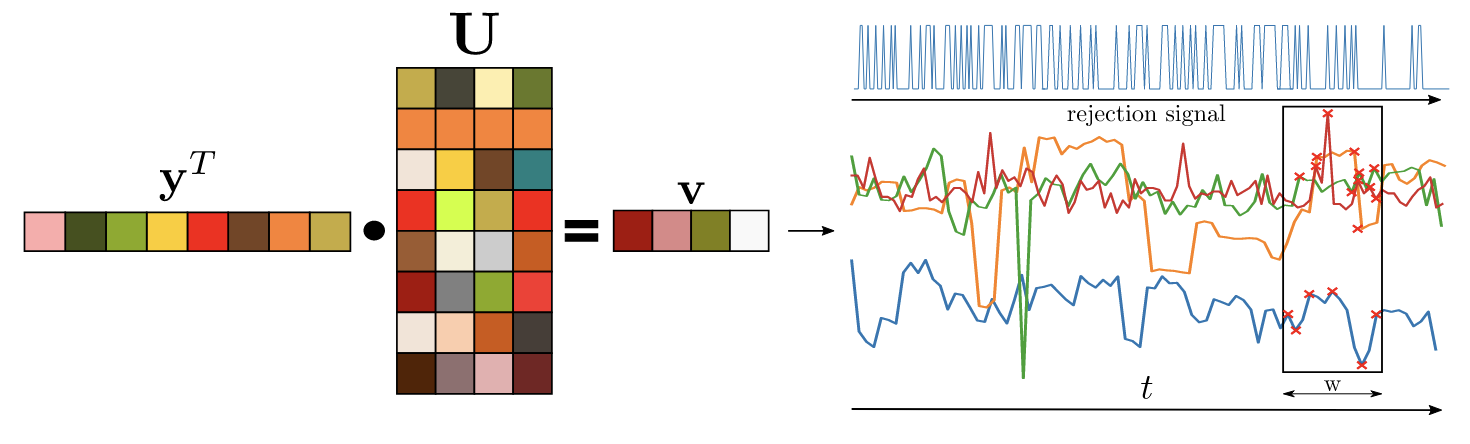
\includegraphics[width=\textwidth]{images/pronto}
    \caption{Projection of incoming $y \in \mathbb{R}^d$ onto embedding $U \in
    \mathbb{R}^{d \times r}$ producing $R$ projections in $v \in \mathbb{R}^{1
    \times r}$. Projections are tracked over time for detecting spikes which
    form the basis of the rejection signal. The sliding window for spike
    detection for each projection is of size $w$ also shown in the figure.}
    \label{pronto-components}
\end{figure}

PCA is a powerful dimensionality reduction technique, used to simplify
complex, high-dimensional datasets while retaining the most information. Pronto
use Federated PCA (a privacy preserving distributed approach to PCA) to extract
features which represent the "directions" with greatest variance. Pronto can
then project telemetry data onto these vector directions to predict future
spikes which indicate resource contention.

Pronto makes use of the following property: The PCA of a matrix can be
calculated by mean centering the data, performing SVD on the resulting matrix to
give $U$, the directions of the principle components, and $\Sigma$ the variance
along these directions. As Pronto aims to be memory-limited, it can't store all
of the collected telemetry and must instead take a streaming approach. It
periodically measures the CPU Ready metric at a given frequency. To perform
FPCA, every new batch of $b$ samples is iteratively merged into the latest
subspace using Incremental-SVD. In addition, to perform global model
aggregation, SVD is performed on the concatenated bases of two local models.
Pronto can further reduce the required computation by using Low-Rank
approximations, reducing the dimensionality to $r$ where $r < m$. It uses the
assumption that the first $r$ eignenvalues contain the majority of the
information of the dataset.

Once a node has a local model, it can periodically generate a signal by
projecting the latest telemetry data onto the principle component subspace $U$
and identifies all the spikes in the projections. If the weighted sum of the
spikes exceeds a threshold, then a rejection signal is raised which indicates
that node is experiencing performance problems and a job should not be
scheduled.

\subsection{Evaluation}

In the Pronto paper, a scheduler's effectiveness was qunatified by its ability
to raise a rejection signal that precedes a CPU-Ready spike within a pre-defined
window, while minimising the number of false positives that do not precede
CPU-Ready spikes. Protono was compared against non-distributed
dimensionality-reduction methods \cite{}, and was shown to predict CPU-Ready
signals effectively while keeping false-positives low. Pronto's better
performance over non-distributed strategies implies that there were correlations
between job's resource usages on different nodes at the same point in time. As a
result, FPCA could use telemetry across multiple nodes to more acurrately
compute the principle components and thus give better CPU-Ready predictions.

These properties make Pronto an attractive technique that could be incorporated
into scheduling within a Kubernetes cluster.

\begin{tcolorbox}[boxsep=0mm,left=2.5mm,right=2.5mm] \textbf{Why Pronto:}
{\em Pronto is promising due to two reasons, its federated nature which could
allow nodes to exploit cluster-level information into their scheduling
decisions, and its use of CPU-Ready, a standard metric to detect contention, but
had not seen use in scheduling}  \end{tcolorbox}

% \begin{tcolorbox}[boxsep=0mm,left=2.5mm,right=2.5mm] \textbf{Subspace Merging:}
% {\em In this chapter I will describe how Pronto builds the indivdual models from
% the \verb|CPU Ready| metric generated by the VMware vSphere platform. I will
% give a brief outline of the matrix operations (SVD) used in Subspace merge
% operations, as well as the Reject Signal generated.} \end{tcolorbox}
%
% \subsection{Strengths \& Weaknesses}
% \begin{tcolorbox}[boxsep=0mm,left=2.5mm,right=2.5mm] \textbf{Strengths \&
% Weaknesses:} {\em In this chapter I outline the strengths and weakness of the
% Pronto approach. Strengths: real-time data allows for prediction of
% system responsiveness allowing for better scheduling decisions and overall
% utilisation. Weaknesses: the original paper does not consider communnication
% latency and task start up latency. This is a challenge as the signal uses
% real-time data and thus requires tasks to have started running to detect future
% spikes.}
% \end{tcolorbox}
%
% \subsection{Theory to Practical}
% \begin{tcolorbox}[boxsep=0mm,left=2.5mm,right=2.5mm] \textbf{Theory to
% Practical:} {\em In this chapter I outline the potential challenges that
% come from implementing a theoretical system. I will outline in more detail
% the issues of real-world communication latencies and how these will effect
% the quality of the generated signal. I will also discuss how the challenges
% of using a signal for scheduling and the need for denoising.} \end{tcolorbox}
%
\section{Summary}
This chapter introduced the core concepts of online scheduling. I explored
existing Kubernetes schedulers, investigating the merits of using pod
description-based schedulers vs. telemetry-based schedulers. From the brief
survey, I identified that few Kubernetes schedulers use deeper contention
indicators, such as cache pressure and memory pressure. Finally, I introduce
Pronto, a novel approach to task scheduling predictor that uses the CPU-Ready
performance metric generated by the VMware vSphere virtualisation platform.

% \begin{tcolorbox}[boxsep=0mm,left=2.5mm,right=2.5mm]
    % \textbf{Summary:} {\em In this chapter I will summarise the problem and
    % problem space. I will review the findings of the related work, highlighting
    % weaknesses of existing Kubernetes schedulesr with respect to QoS
    % scheduling.}
% \end{tcolorbox}

